\documentclass[xcolor=table]{beamer}
\usepackage{etex}
\usepackage[absolute,overlay]{textpos}
\usepackage{lmodern}
\usepackage[T1]{fontenc}
\usepackage[utf8]{inputenc}
\usepackage[magyar]{babel}
\usepackage{standalone}
\usepackage{adjustbox}
\usepackage{varwidth}
\usepackage{tikz}

\usetikzlibrary{shapes, positioning, mindmap, arrows.meta, backgrounds, fit}
\newcommand{\tikzmark}[1]{\tikz[overlay,remember picture] \node (#1) {};}

\setbeamercolor{framesource}{fg=gray}
\setbeamerfont{framesource}{size=\tiny}

% straight from http://tex.stackexchange.com/a/55849/8785
  \tikzset{
    invisible/.style={opacity=0},
    visible on/.style={alt={#1{}{invisible}}},
    alt/.code args={<#1>#2#3}{%
      \alt<#1>{\pgfkeysalso{#2}}{\pgfkeysalso{#3}} % \pgfkeysalso doesn't change the path
    },
  }
\title{A PLanG programozási nyelv kiterjesztése}
\subtitle{Önálló laboratóriumi beszámoló}
\author{Scipiades Ármin\\\bigskip Konzulens: Dr.\thinspace Feldhoffer Gergely}
\date{2015. május 27.}

\usetheme{Rochester}
\usecolortheme{beaver}
\setbeamertemplate{navigation symbols}{}

\newcommand{\source}[1]{\begin{textblock*}{4cm}(8.7cm,9cm)
    \begin{beamercolorbox}[ht=0.5cm,right]{framesource}
        \usebeamerfont{framesource}\usebeamercolor[fg]{framesource}{#1}
    \end{beamercolorbox}
\end{textblock*}}

\begin{document}

\frame{\titlepage}

\begin{frame}
	\frametitle{A PLanG programozási nyelv}
	\centering
	\includegraphics[width=\linewidth,height=\textheight,keepaspectratio]{images/plang.pdf}
\end{frame}

\begin{frame}
	\frametitle{A PLanG hiányosságai}
	\centering
	\begin{adjustbox}{max totalsize={\textwidth}{\textheight},center}
	\begin{tikzpicture}[
	box/.style = {fill=#1!20,draw=#1, rounded corners, inner sep=2mm, very thick}
]
\node[text width=10cm, opacity=0.4, anchor=south west, inner sep=0, visible on=<1->] (bg) {{\includestandalone[width=\textwidth]{images/skull_and_crossbones}}};

\begin{scope}[x={(bg.south east)},y={(bg.north west)}]

\node[box=yellow, anchor=north west, visible on=<2->] at (0.37,0.85) {%
\begin{varwidth}{\linewidth}
\begin{verbatim}
Változók: a, b: Szöveg
  ...
  Ki: a @ b
\end{verbatim}
\end{varwidth}
%
};


\node[box=orange, anchor=north west, visible on=<3->] at (0.25,0.79) {%
\begin{varwidth}{\linewidth}
\begin{verbatim}
	Ha x akkor
	  ki: "igaz ág"
	különben
	  ha y akkor
	    ki: "nem x és y"
	  különben
	    ha z akkor
	      ki: "nem x és nem y és z"
      különben
        ki: "semmi nem igaz"
	    ha_vége
	  ha_vége
	ha_vége
\end{verbatim}
\end{varwidth}
%
};

\node[box=red, anchor=north west, visible on=<4->] at (-0.1,0.92) {%
\begin{varwidth}{\linewidth}
\begin{verbatim}
  ha x akkor
    ** x-re vonatkozó helyes viselkedés
    ha y akkor
      ** y-ra vonatkozó helyes viselkedés
    különben
      ki: "Hiba: y nem igaz"
  különben
    ki: "Hiba: x nem igaz"
  ha_vége
\end{verbatim}
\end{varwidth}
%
};

\node[box=purple, anchor=north west, visible on=<5->] at (0.1,0.65) {%
\begin{varwidth}{\linewidth}
\begin{verbatim}
  ...függvény meg egyáltalán nincs...
\end{verbatim}
\end{varwidth}
%
};

\end{scope}
\end{tikzpicture}

	\end{adjustbox}
\end{frame}

\begin{frame}
	\frametitle{Objektív értékelés?}
	\centering
	\includegraphics{images/subjective_kloran.png}
	
	\source{Michael Kloran illusztrációja}
\end{frame}

\begin{frame}
	\frametitle{A programozási nyelv felhasználói felület}	
	\centering
	\begin{adjustbox}{max totalsize={\textwidth}{\textheight},center}
	\begin{tikzpicture}[
	node distance=10cm,
	stuff/.style={draw, cloud, cloud ignores aspect, font=\Huge},
	img/.style={text width=3cm, minimum height=3cm},
	arr/.style={->, >={Latex[length=0.4cm]}, shorten >=1pt},
	label/.style={fill=white, font=\Huge}
]

\node[stuff] (input) {Feladat};
\node[img, below= 3cm of input] (human) {{\includestandalone[width=\textwidth]{images/human_head}}};
\node[img, right of=human, text width=6cm] (language) {{\includegraphics[width=\textwidth]{images/plang.pdf}}};
\node[img, right of=language] (computer) {{\includestandalone[width=\textwidth]{images/computer}}};
\node[stuff, above=3cm of computer] (output) {Megoldás};

\draw[arr] (input) edge (human);
\draw[arr] (human) edge node[label] {algoritmus} (language);
\draw[arr] (language) edge node[label] {program} (computer);
\draw[arr] (computer) edge (output);

\end{tikzpicture}

	\end{adjustbox}	
\end{frame}

\begin{frame}
	\frametitle{Programozási nyelvek minőségi mutatói}
	\centering
	\begin{adjustbox}{max totalsize={\textwidth}{\textheight},center}
	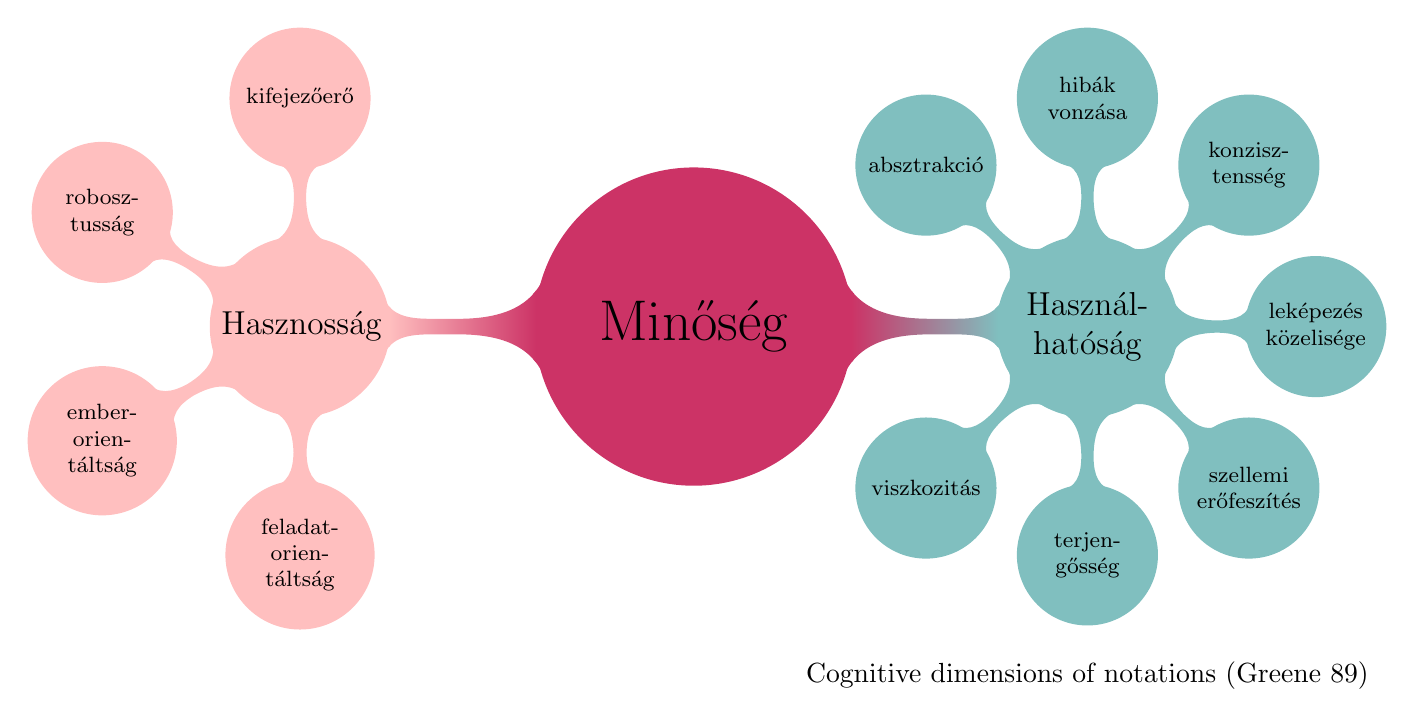
\begin{tikzpicture}
	\path[
		mindmap,
		concept color=purple!80,
		text=black
	]
		node [concept, font=\huge] {Minőség}
		[clockwise from=0, level 1 concept/.append style={sibling angle=180}]
		child[concept color=teal!50] {
			node[concept, font=\large] (usability) {Hasz\-nál\-ha\-tó\-ság}
			[clockwise from=135, level 2 concept/.append style={sibling angle=45, visible on=<3->}]
			child { node[concept] {absztrakció} }
			child { node[concept] {hibák vonzása} }
			child { node[concept] {kon\-zisz\-tens\-ség} }
			child { node[concept] {leképezés közelisége} }
			child { node[concept] {szellemi erőfeszítés} }
			child { node[concept] {ter\-jen\-gős\-ség} }
			child { node[concept] {viszkozitás} }
		}
		child[concept color=pink] {
			node[concept, font=\large] {Hasznosság}
			[counterclockwise from=90, level 2 concept/.append style={sibling angle=60, visible on=<2->}]
			child { node[concept] {ki\-fe\-je\-ző\-e\-rő} }
			child { node[concept] {ro\-bosz\-tus\-ság} }
			child { node[concept] {ember\-orien\-táltság} }
			child { node[concept] {feladat\-orien\-táltság} }
		};

		\node[below=3 of usability, visible on=<3->] {Cognitive dimensions of notations (Greene 89)};
\end{tikzpicture}

	\end{adjustbox}
\end{frame}

\begin{frame}
	\frametitle{A PLanG minőségi mutatói}
	\centering
	\begin{tabular}{ r c c }
\bfseries kognitív dimenzió						& \bfseries PLanG	 & \bfseries ideális oktatási nyelv  \\
\rowcolor{red!30}		\bfseries absztrakció 		&nincs & alacsony \\
\rowcolor{red!30}		\bfseries hibák vonzása 	&közepes & nagyon alacsony \\
\rowcolor{green!30}		\bfseries konzisztensség 	&közepes & közepes  \\
\rowcolor{red!30}		\bfseries leképezés közelisége &közepes-alacsony & nagyon magas \\
\rowcolor{red!30}		\bfseries szellemi erőfeszítés &közepes & alacsony \\
\rowcolor{yellow!30}		\bfseries szerepkifejezés &közepes-magas	& magas \\
\rowcolor{yellow!30}		\bfseries terjengősség &alacsony-közepes	& közepes \\
\rowcolor{red!30}		\bfseries viszkozitás &közepes-magas	& alacsony
	\end{tabular}
\end{frame}


\begin{frame}
	\frametitle{Parametrizálható fordítóprogram}
	\centering
	\begin{adjustbox}{max totalsize={\textwidth}{\textheight},center}
	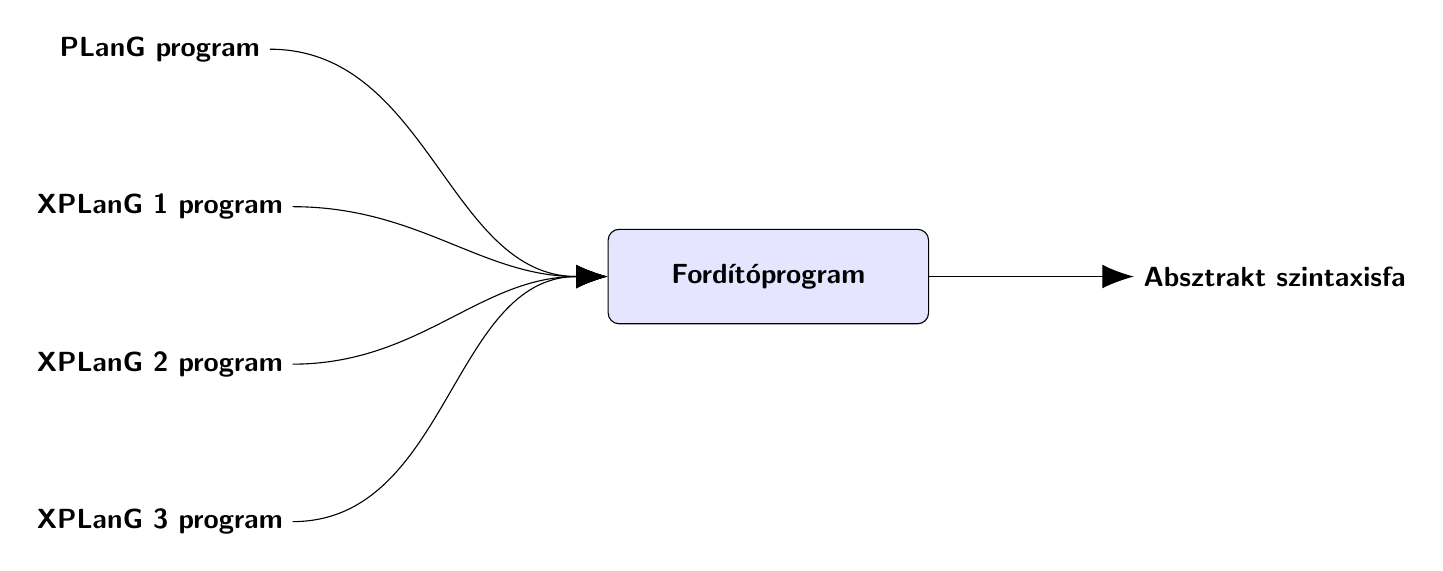
\begin{tikzpicture}[node distance=2cm,
	every node/.style={font=\bfseries\sffamily},
	clas/.style={rectangle, rounded corners, draw, fill=blue!10, inner sep=1pt, text width=4cm, text badly centered, minimum height=1.2cm},
	arr/.style={->, >={Latex[length=0.4cm]}}
	]

\node (1es) {PLanG program};
\node[below of=1es] (2es) {XPLanG 1 program};
\node[below of=2es] (3as) {XPLanG 2 program};
\node[below of=3as] (4es) {XPLanG 3 program};

\node[clas, below right=0cm and 4cm of 2es] (interpreter) {Fordítóprogram};

\node[right=2.6cm of interpreter] (out) {Absztrakt szintaxisfa};

\path[arr]
(1es) edge[out=0, in=180] (interpreter)
(2es) edge[out=0, in=180] (interpreter)
(3as) edge[out=0, in=180] (interpreter)
(4es) edge[out=0, in=180] (interpreter)
(interpreter) edge (out);


\end{tikzpicture}

	\end{adjustbox}
\end{frame}

\begin{frame}
	\frametitle{A prototípus adatfolyam diagramja}
	\centering
	\begin{adjustbox}{max totalsize={\textwidth}{\textheight},center}
	\begin{tikzpicture}[node distance=1cm,
	every node/.style={node distance=2cm, },
	clas/.style={rectangle, rounded corners, draw, fill=blue!10, inner sep=1pt, text width=2.4cm, text badly centered, minimum height=1.2cm, font=\bfseries\sffamily},
	arr/.style={->, >=latex', shorten >=1pt}
	]

\node[clas] (parser) {Parser};
\node[clas, above=of parser] (grammar) {Grammar};
\node[clas, left=of parser] (lexer) {Lexer};
\node[clas, below left=2 and 1 of parser] (context) {Context};
\node[clas, below right=2 and 1 of parser] (typechecker) {Typechecker};

\node[clas, left=of lexer] (source) {Forrásszöveg};
\node[clas, right=of parser] (interpreter) {AST Interpreter};

\path[arr, every node/.style={font=\itshape\footnotesize,
  		fill=white,inner sep=3pt}]
(source) edge node[above] {karakterek} (lexer)
(parser) edge [bend left=30] node {új állapot} (context)
(context) edge[bend left=30] node {állapot} (parser)
(grammar) edge node[above] {szabály} (parser)
(lexer) edge  node[above] {tokenek} (parser)
(parser) edge[bend right=30] node {AST-node} (typechecker)
(typechecker) edge[bend right=30] node {helyes AST-node} (parser)
(context) edge[bend right=15] node {állapot} (typechecker)
(parser) edge node[above] {AST} (interpreter);

\end{tikzpicture}

	\end{adjustbox}
\end{frame}


\begin{frame}[fragile]
	\frametitle{XPLanG}
	\centering
	\begin{adjustbox}{max totalsize={\textwidth}{\textheight},center}
	\begin{tikzpicture}[
	box/.style = {fill=#1!20,draw=#1, rounded corners, inner sep=2mm, very thick}
]
\node[anchor=south west,inner sep=0] (bg) at (0,0) {\includestandalone[width=10cm]{images/cute_cloud}};

\begin{scope}[x={(bg.south east)},y={(bg.north west)}]


\node[box=blue, anchor=north west, visible on=<2->] at (-0.1,0.92) {%
\begin{varwidth}{\linewidth}
\begin{verbatim}
	Függvény faktoriális (n: Egész) => Eredmény: Egész
	  Eredmény := n
	  ciklus amíg n>2
	    n := n-1
	    Eredmény := Eredmény * n
	  ciklus_vége
	Függvény_vége
\end{verbatim}
\end{varwidth}
%
};

\node[box=green, anchor=north west, visible on=<3->] at (-0.05,0.87) {%
\begin{varwidth}{\linewidth}
\begin{verbatim}
	Ha x akkor
	  ki: "igaz ág"
	vagy_ha y akkor
	  ki: "elsif ág"
	vagy_ha z akkor
	  ki: "másik elsif ág"
	különben
	  ki: "else ág"
	ha_vége
\end{verbatim}
\end{varwidth}
%
};

\node[box=teal, anchor=north west, visible on=<4->] at (0,0.82) {%
\begin{varwidth}{\linewidth}
\begin{verbatim}
	Ha nem x akkor
	  hiba: "x nem igaz"
	ha_vége
\end{verbatim}
\end{varwidth}
%
};


\end{scope}

\end{tikzpicture}

	\end{adjustbox}
\end{frame}

\begin{frame}
	\frametitle{Összegzés}
	\begin{itemize}
		\item Minőségi mutatók programozási nyelvekhez
		\item A PLanG minőségi mutatói nem túl jók
		\item XPLanG: alprogramok, többágú elágazás, hibakezelés
		\item Nyelvtannal paraméterezhető fordítóprogram: sok lehetőség
	\end{itemize}
\end{frame}
\end{document}